% !TeX spellcheck = fr_FR
\chapter{Chapitre 5 : Analyse des résultats}

Ce chapitre présente une lecture approfondie — mais accessible et agréable — de la qualité de nos correspondances ATLAS $\leftrightarrow$ OSM. Nous mêlons graphiques, petits extraits de code et indicateurs lisibles, avec une attention particulière aux cas limites et aux pistes d'amélioration.

\section{Comment nous avons calculé les statistiques}

Nous utilisons directement la base MySQL du projet (variable d'environnement \texttt{DATABASE\_URI}). Les scripts sont fournis et versionnés sous \texttt{memoire/scripts\_used/chap5}. Voici un minuscule extrait montrant le chargement des données et le calcul de statistiques par méthode de 
correspondance:

\begin{verbatim}
# memoire/scripts_used/chap5/chap5_distance_distributions.py (extrait)
engine = create_engine(os.getenv('DATABASE_URI', 'mysql+pymysql://...'))
df = pd.read_sql(
    """
    SELECT distance_m, match_type, osm_node_type
    FROM stops
    WHERE stop_type = 'matched' AND distance_m IS NOT NULL
    """, engine)
summary = (
  df.groupby('match_type')['distance_m']
    .agg(count='count', mean='mean', median='median')
    .reset_index()
)
summary.to_csv('.../distance_summary_by_method.csv', index=False)
\end{verbatim}

Tous les chiffres et graphiques de ce chapitre sont produits par ces scripts, exécutés sur la base actuelle.

\section{Distribution des distances par méthode}

\begin{figure}[h]
    \centering
    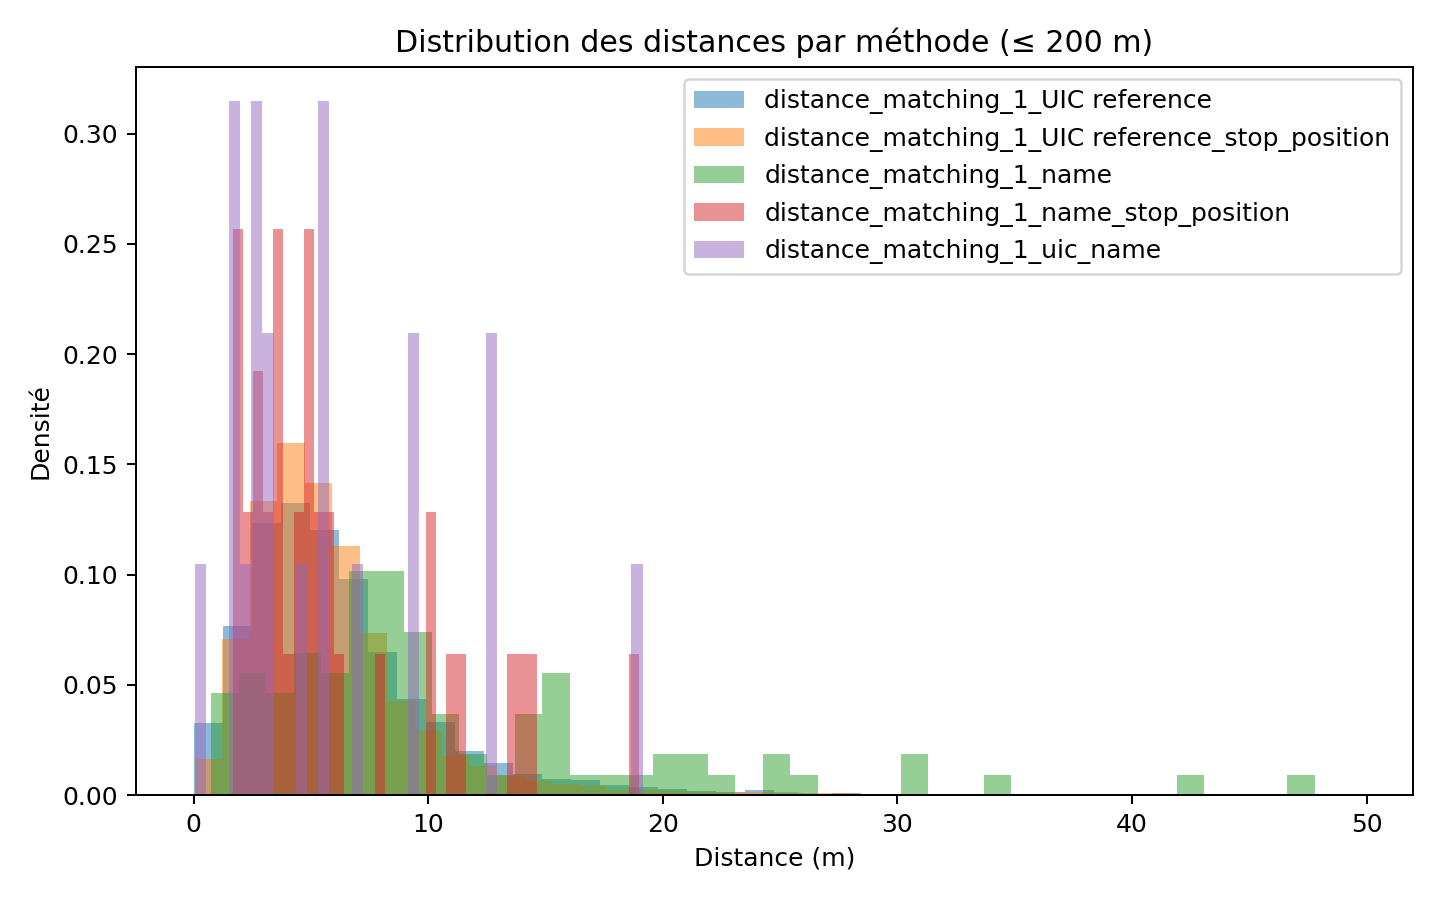
\includegraphics[width=\textwidth]{../figures/chap5/distances_by_method_hist_0_200.png}
    \caption[Distances par méthode ($\leq$ 200 m)]{Distribution des distances par méthode de correspondance (coupée à 200 m pour mieux voir le cœur).}
\end{figure}

\begin{figure}[h]
    \centering
    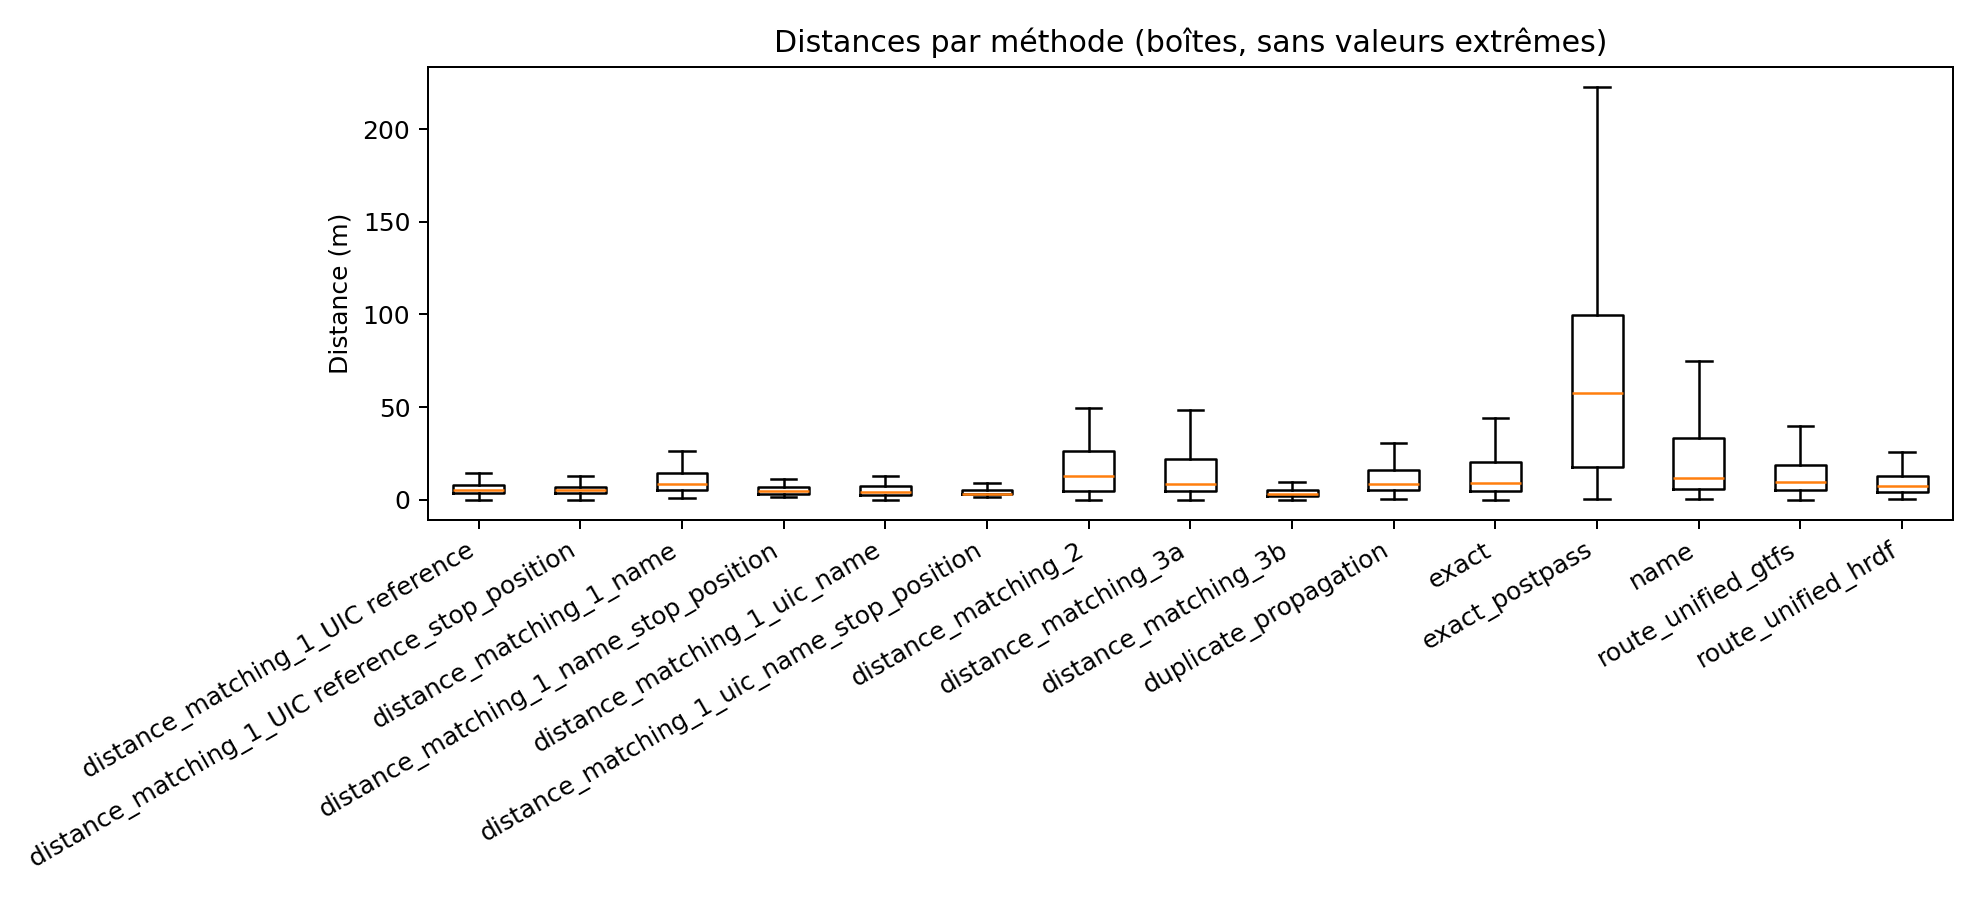
\includegraphics[width=\textwidth]{../figures/chap5/distances_by_method_box.png}
    \caption[Boîtes par méthode]{Boîtes à moustaches par méthode (sans valeurs extrêmes) — lecture immédiate des médianes et de la dispersion.}
\end{figure}

\begin{figure}[h]
    \centering
    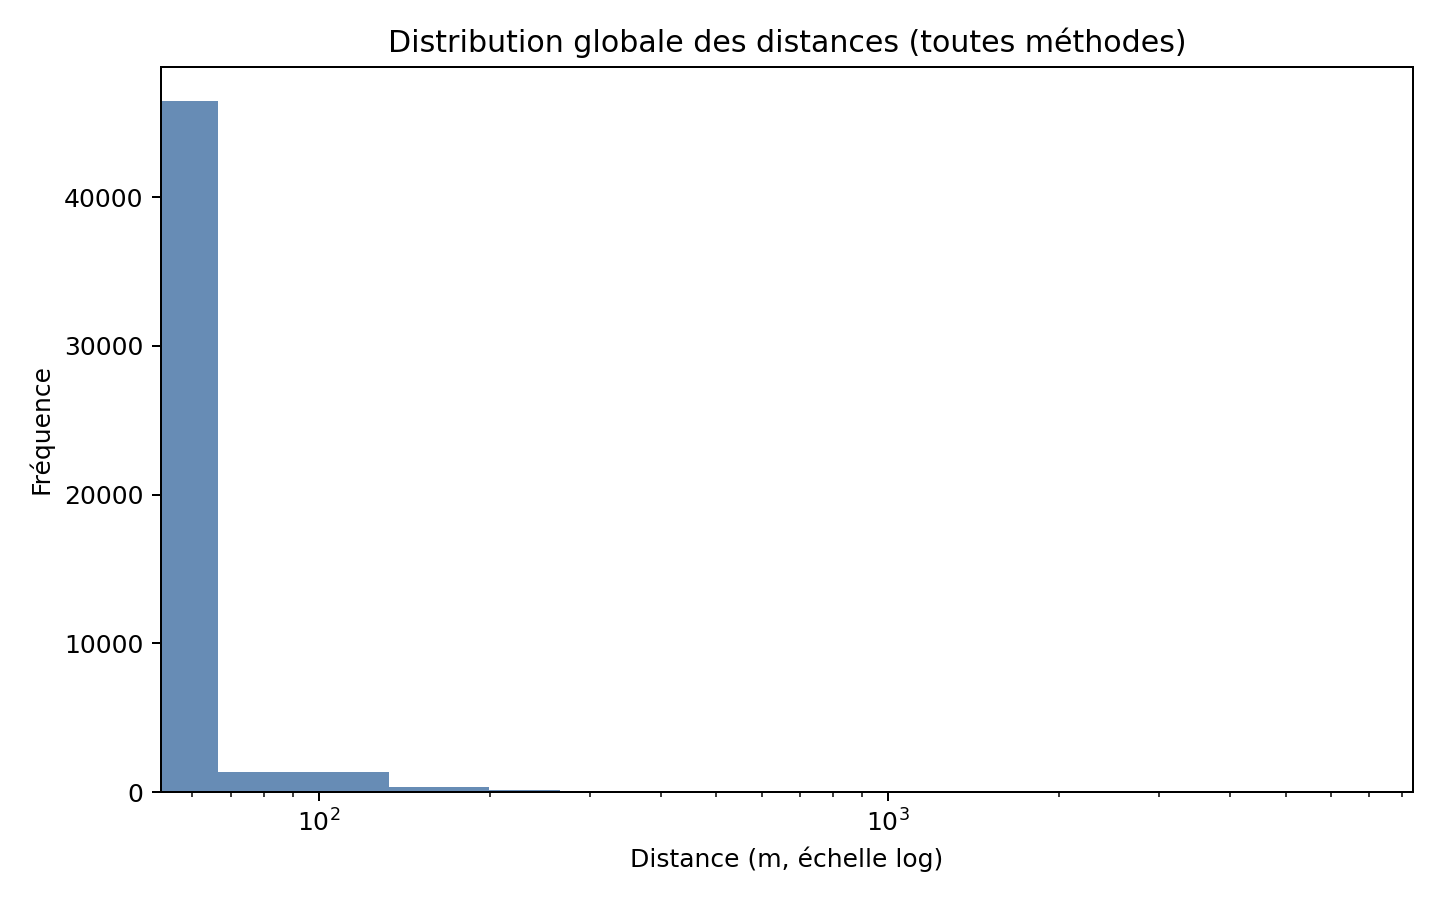
\includegraphics[width=\textwidth]{../figures/chap5/distances_global_hist.png}
    \caption[Distribution globale (log)]{Distribution globale des distances (échelle logarithmique) — utile pour visualiser la longue traîne.}
\end{figure}

\noindent Extraits des résultats par méthode (fichier \texttt{distance\_summary\_by\_method.csv}) :

\begin{verbatim}
match_type,count,mean,median,p90,p95,p99,pct_<=10m,pct_<=20m,pct_<=50m,pct_<=100m
exact,21250,22.28,9.10,51.24,82.36,207.28,53.6%,74.4%,89.7%,96.4%
route_unified_gtfs,4348,13.95,9.70,32.98,40.76,47.96,51.6%,75.6%,100%,100%
route_unified_hrdf,2769,10.30,7.10,23.19,31.10,45.04,65.8%,86.4%,100%,100%
distance_matching_3b,1191,3.70,3.28,6.83,8.00,10.09,98.9%,100%,100%,100%
... (voir CSV complet)
\end{verbatim}

Points saillants:
\begin{itemize}
    \item Les méthodes « distance \texttt{3b} » et « distance (UIC/stop\_position) » sont extrêmement précises (médianes \(\approx\) 3–5 m).
    \item Les « exacts » recouvrent des cas hétérogènes: médiane correcte (\(\approx\) 9 m) mais longue traîne liée aux homonymies et ancrages OSM imparfaits.
    \item Les unifications de lignes GTFS/HRDF sont globalement saines (médianes \(\approx\) 7–10 m), avec une dispersion modérée.
\end{itemize}

\section{Par opérateur: où est-ce le plus précis ?}

Nous joignons chaque arrêt à son opérateur ATLAS et analysons les distances des arrêts 
\textit{matchés}. Nous affichons ici un classement visuel des opérateurs les plus représentés.

\begin{figure}[h]
    \centering
    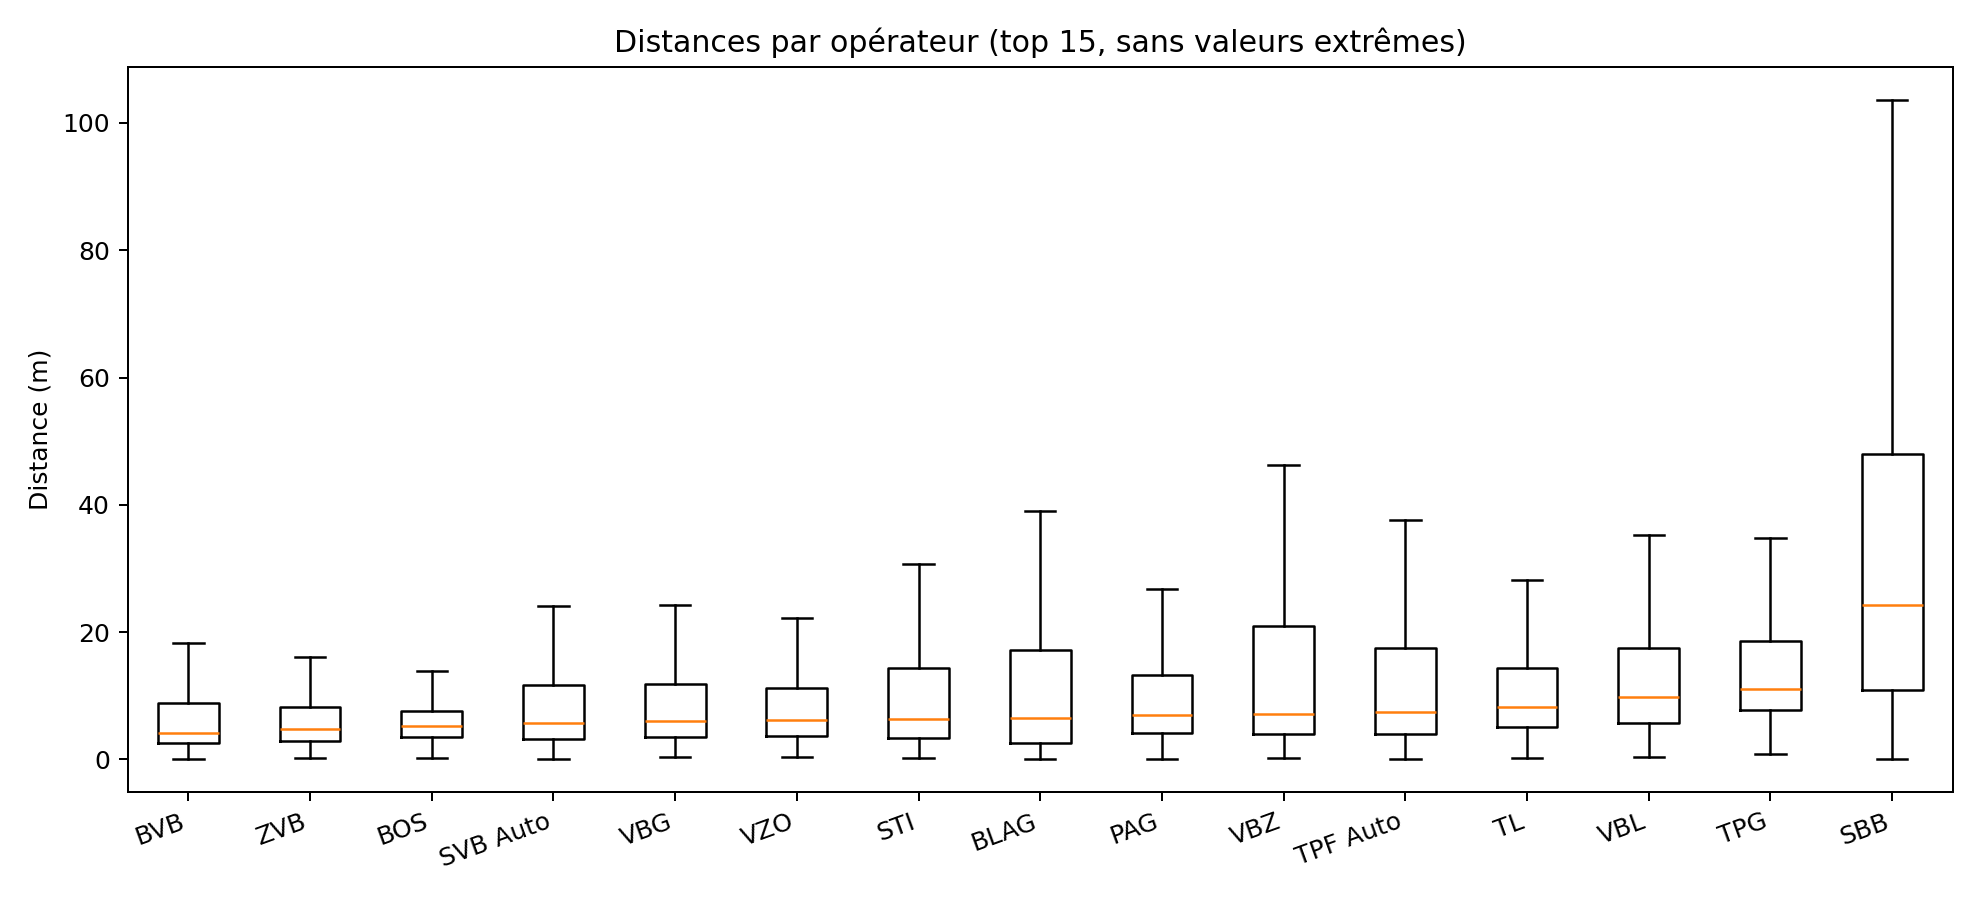
\includegraphics[width=\textwidth]{../figures/chap5/distances_by_operator_box.png}
    \caption[Distances par opérateur]{Dispersion des distances par opérateur (top 15 par effectif).}
\end{figure}

Observations rapides:
\begin{itemize}
    \item Les opérateurs urbains à forte densité de données (p. ex. \texttt{TPG}, \texttt{VBZ}, \texttt{PAG}) présentent des médianes de l'ordre de 7–12 m, cohérentes avec un calage cartographique fin.
    \item Certains opérateurs de montagne ou réseaux spéciaux montrent des dispersions plus larges — terrain complexe, géoréférencement moins standardisé.
\end{itemize}

\section{Les non-matchés et leurs \og alter ego \fg{} proches}

Combien d'entrées non-correspondantes ont pourtant un arrêt matché à proximité ? Nous échantillonnons 
des rayons de 25, 50, 100, 200 et 400 m autour de chaque non-matché (sur coordonnées ATLAS).

\begin{verbatim}
radius_m,unmatched_total,with_nearby_counterpart,pct
25,9537,1946,20.40
50,9537,2744,28.77
100,9537,3192,33.47
200,9537,3195,33.50
\end{verbatim}

Donc \textbf{entre 20\% et 34\%} des non-matchés ont un correspondant plausible très proche. Deux scénarios fréquents: (i) doublon/homonymie ATLAS à consolider ; (ii) ancrage OSM 
existant mais filtré (type de nœud, règles). Ces cas sont d'excellents candidats à la remédiation semi-automatique.

\section{Autres statistiques utiles}

\subsection*{Répartition par tranches de distance}

\begin{figure}[h]
    \centering
    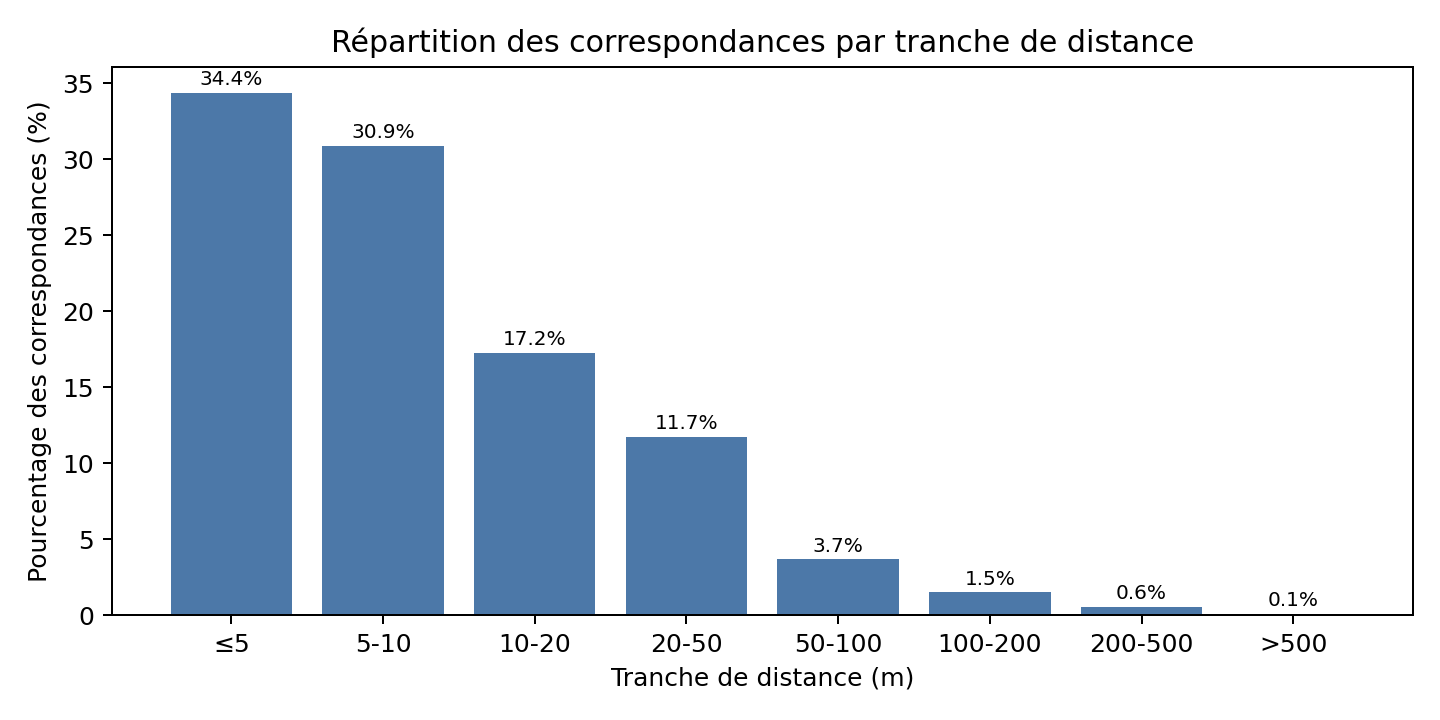
\includegraphics[width=0.9\textwidth]{../figures/chap5/distance_coverage_buckets.png}
    \caption[Tranches de distance]{Quelle part des correspondances tombent sous 5 m, 10 m, 20 m, etc.}
\end{figure}

Cette vue permet d'orienter des objectifs de qualité (p. ex. \og 80\% \(\leq\) 10 m \fg{}).

\subsection*{Surveiller la traîne longue}

Nous listons également les correspondances \(>\) 300 m (\texttt{suspicious\_long\_distances.csv}). 
Cela représente \texttt{111} cas à reclasser en priorité (erreur de rattachement, homonymie distante, etc.).

\section{Mini recettes reproductibles}

\begin{verbatim}
# Distances par type de nœud OSM (extrait)
subset = df[df['osm_node_type'].fillna('inconnu').isin(top_types)]
order = subset.groupby('osm_node_type')['distance_m']\
         .median().sort_values().index.tolist()
plt.boxplot([subset[subset['osm_node_type']==t]['distance_m'] for t in order],
            labels=order, showfliers=False)
\end{verbatim}

\begin{figure}[h]
    \centering
    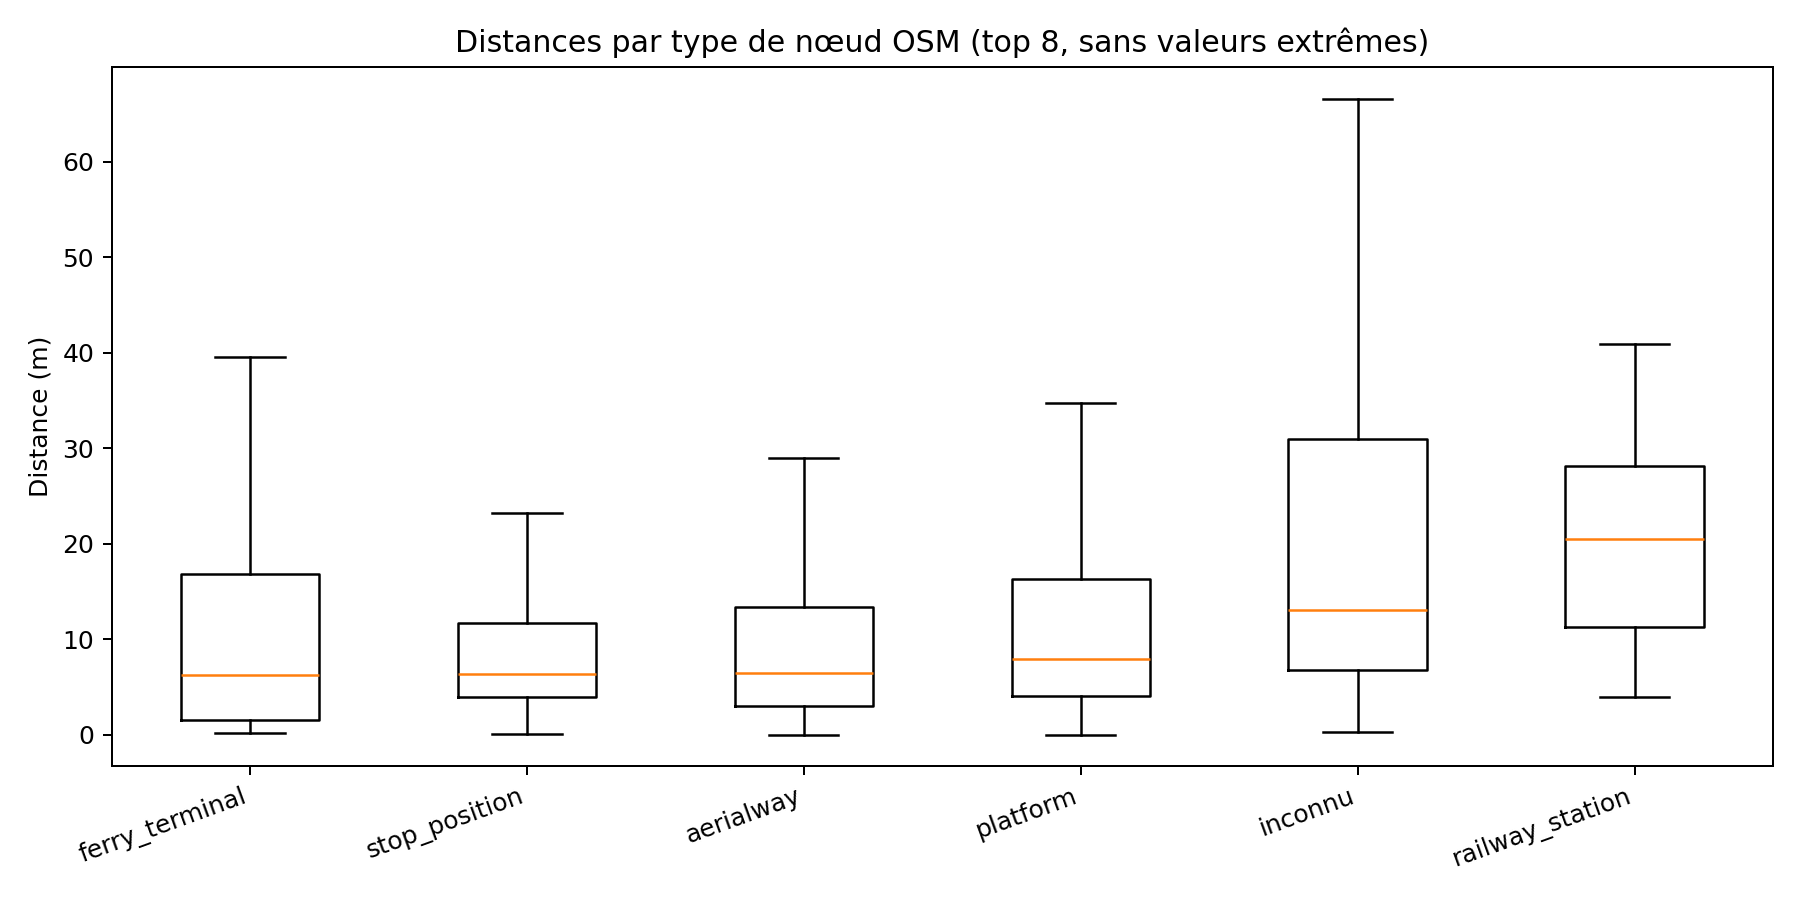
\includegraphics[width=\textwidth]{../figures/chap5/distances_by_osm_node_type_box.png}
    \caption[Par type de nœud OSM]{Certains types (\texttt{stop\_position}, \texttt{platform}) resserrent nettement les distances.}
\end{figure}

\section{Réflexions et pistes d'amélioration}

\begin{itemize}
    \item \textbf{Homonymies et \og exacts \fg{} éloignés} — compléter la règle par des garde-fous spatiaux simples (ex.: rejet si \(>\) 1 km) et par une disambiguation toponymique (commune, canton).
    \item \textbf{Propagation contrôlée des doublons} — les cas \og duplicate\_propagation \fg{} doivent être bornés spatialement et validés à l'échelle du couloir de ligne.
    \item \textbf{Voisinage des non-matchés} — les \(20\)–\(35\%\) proches d'un match peuvent bénéficier d'une auto-suggestion (\og propose un rattachement \fg{}) avec validation humaine.
    \item \textbf{Boucle de qualité continue} — mettre en place des seuils cibles (\(\leq\) 10 m pour 80\% des cas, \(\leq\) 50 m pour 95\%) et un tableau de bord hebdomadaire.
    \item \textbf{Spécificités opérateurs/terrain} — affiner les heuristiques selon les familles d'opérateurs (urbain, montagne, lacustre) et les types de nœuds OSM les plus fiables.
\end{itemize}

En résumé, l'alignement est globalement bon (médianes \(\leq\) 10 m pour les méthodes robustes), avec une traîne que l'on sait désormais 
localiser et traiter. Les scripts livrés rendent ces constats reproductibles et extensibles.

